\documentclass[letter,11pt]{article}

\usepackage[spanish,es-nodecimaldot]{babel}
\usepackage[utf8]{inputenc}

\usepackage{lmodern}
\usepackage[T1]{fontenc}
\usepackage{textcomp}

\usepackage{framed}
\usepackage[svgnames]{xcolor}
\colorlet{shadecolor}{Gainsboro!50}

\usepackage[labelfont=bf]{caption}
\usepackage{graphicx}
\usepackage{pstricks}

\usepackage{anysize}
\marginsize{3cm}{2cm}{2cm}{3cm}

\usepackage{url}
\usepackage{siunitx}
\usepackage{amsmath}
\usepackage{array}
\usepackage{alltt}
\usepackage{xcolor,colortbl}

\usepackage{fancyhdr}
\usepackage{lastpage}
\pagestyle{fancy}
\fancyhf{}
\fancyhead[LE,RO]{Laboratorio de Física Básica III}
\fancyfoot[CO,CE]{\thepage\ de \pageref{LastPage}}

\special{papersize=215.9mm,279.4mm}

\usepackage[
    pdfauthor={
        Bastos Lizondo Rosemary;
        Blanco Alconz John Brandon;
        Caballero Burgoa Carlos Eduardo;
        Villena Gutiérrez Ismael Cristian
    },%
    pdftitle={Laboratorio de Física Básica III},%
    pdfsubject={Condensador plano o de placas paralelas},%
    colorlinks,%
    citecolor=black,%
    filecolor=black,%
    linkcolor=black,%
    urlcolor=black,
    breaklinks]{hyperref}
\usepackage{breakurl}

\newcommand{\blankpage}{
\newpage
\thispagestyle{empty}
\mbox{}
\newpage
}

\renewcommand{\arraystretch}{1.2}

\begin{document}

\begin{titlepage}
\begin{center}
{\Large UNIVERSIDAD MAYOR DE SAN SIMÓN}\\
\vspace*{0.15cm}
{\large FACULTAD DE CIENCIAS Y TECNOLOGÍA}\\
\vspace*{0.10cm}
DEPARTAMENTO DE FÍSICA\\
\vspace*{3.0cm}
{\Large \textbf{LABORATORIO DE FÍSICA BÁSICA III}}\\
\vspace*{0.3cm}
{\Large \textbf{INFORME No. 5}}\\
\vspace*{3.5cm}
{\Large \textbf{CONDENSADOR PLANO \\O DE PLACAS PARALELAS}}\\
\end{center}

\vspace*{5.8cm}
\leftskip=7.95cm
\noindent
\textbf{Integrantes:}\\
Bastos Lizondo Rosemary.\\
Blanco Alconz John Brandon.\\
Caballero Burgoa Carlos Eduardo.\\
Villena Gutiérrez Ismael Cristian.\\
\newline
\textbf{Docente:}\\
Ing. Flores Flores, Freddy.\\
\newline
\textbf{Grupo:} G3.\\
\textbf{Fecha de entrega:} 21 de Abril del 2021.\\

\end{titlepage}

\section{Objetivos}
\begin{itemize}
\item Encontrar la relación funcional entre la capacitancia en función de la
    distancia.
\item Encontrar la relación funcional entre la capacitancia en función del área.
\item Encontrar el valor de la permitividad del vacío.
\end{itemize}

\section{Fundamento teórico}

Dos conductores, aislados eléctricamente uno del otro que tienen una diferencia
de potencial $V_{ab}$ entre ellos y que tienen cargas iguales y opuestas. Se
denomina capacitor o condensador (\textbf{Figura \ref{figura1}}).

\begin{figure}[!h]
\centering
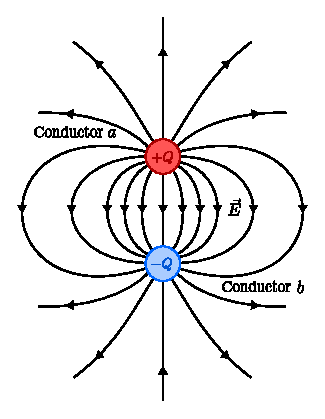
\includegraphics[scale=1.00]{resources/f1.eps}
\caption{Dos conductores cualesquiera $a$ y $b$ \\ aislados uno del otro forman
un capacitor.}
\label{figura1}
\end{figure}

La capacitancia o capacidad de un capacitor se define como la razón entre la
magnitud de la carga en cualquiera de los conductores y la magnitud de la
diferencia de potencial entre ellos:

\begin{equation}
    C = \frac{Q}{V_{ab}}
\label{capacitancia}
\end{equation}

En la medida que aumenta la magnitud de la carga en los conductores aumenta
también la diferencia de potencial entre ellos, pero el cociente $Q/V_{ab}$ se
mantiene constante para un capacitor dado.

La unidad del SI para la capacitancia es el \emph{Faradio} ($1 [F]$), en honor
del físico inglés del siglo XIX, \emph{Michael Faraday}. De acuerdo con la
\textbf{Ecuación (\ref{capacitancia})}, un \emph{Faradio} es igual a un
\emph{Coulomb} por \emph{Voltio} ($1 [C/V]$):

\begin{equation}
    1 [F] = 1 \left[\frac{C}{V}\right]
\label{faradio}
\end{equation}

El tipo más sencillo de capacitor consiste en dos placas conductoras paralelas,
cada una con área $A$, separadas por una distancia $d$ que es pequeña en
comparación con sus dimensiones (\textbf{Figura \ref{figura2}}).

\begin{figure}[!h]
\centering
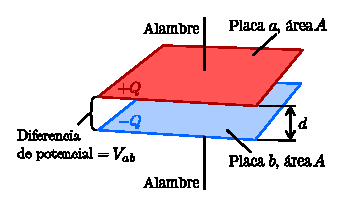
\includegraphics[scale=1.20]{resources/f2.eps}
\caption{Arreglo de placas del capacitor.}
\label{figura2}
\end{figure}

Cuando las placas tienen carga, el campo eléctrico está localizado casi por
completo en la región entre las placas. El campo entre esas placas es
esencialmente uniforme, y las cargas en las placas se distribuyen de manera
uniforme en las superficies opuestas. Este arreglo recibe el nombre de capacitor
de placas paralelas.

Dos placas paralelas de igual área $A$ están separadas una distancia $d$ como en
la \textbf{Figura \ref{figura2}}. Una placa tiene carga $+Q$, y la otra, carga
$-Q$. Utilizando el teorema de \emph{Gauss}, la carga por unidad de área en cada
placa es $Q/A$. Si las placas están muy cercanas una de la otra, podemos
despreciar los efectos de los extremos y suponer que el campo eléctrico es
uniforme entre las placas y el campo eléctrico entre las placas está dado por:

\begin{equation}
    E = \frac{\sigma}{\epsilon_0} = \frac{Q}{\epsilon_0 A}
\label{campoelectrico}
\end{equation}

La diferencia de potencial entre las placas es igual a $E d$; por lo tanto:

\begin{equation}
    V = E d = \frac{Q d}{\epsilon_0 A}
\label{voltaje}
\end{equation}

Sustituyendo este resultado, encontramos que la capacitancia está dada por:

\begin{equation}
    C = \frac{Q}{V} = \epsilon_0 \frac{A}{d}
\label{capacitancia}
\end{equation}

Esto significa que la capacitancia de un condensador de placas paralelas es
proporcional al área $A$ de éstas e inversamente proporcional a la separación
$d$ entre ellas.

\section{Materiales}
\begin{itemize}
\item Simulador «PhET Interactive Simulations» Lab de condensadores: Intro.
\end{itemize}

\section{Procedimiento experimental}
A continuación se describe el procedimiento experimental que se llevará a cabo:

\subsection{Capacitancia en función de la distancia}

\begin{enumerate}
\item Ir al simulador ubicado en la dirección web:
    \url{https://phet.colorado.edu/sims/html/capacitor-lab-basics/latest/capacitor-lab-basics_es.html},
        tal como se muestra en la \textbf{Figura \ref{figura3}}.

\begin{figure}[!h]
\centering
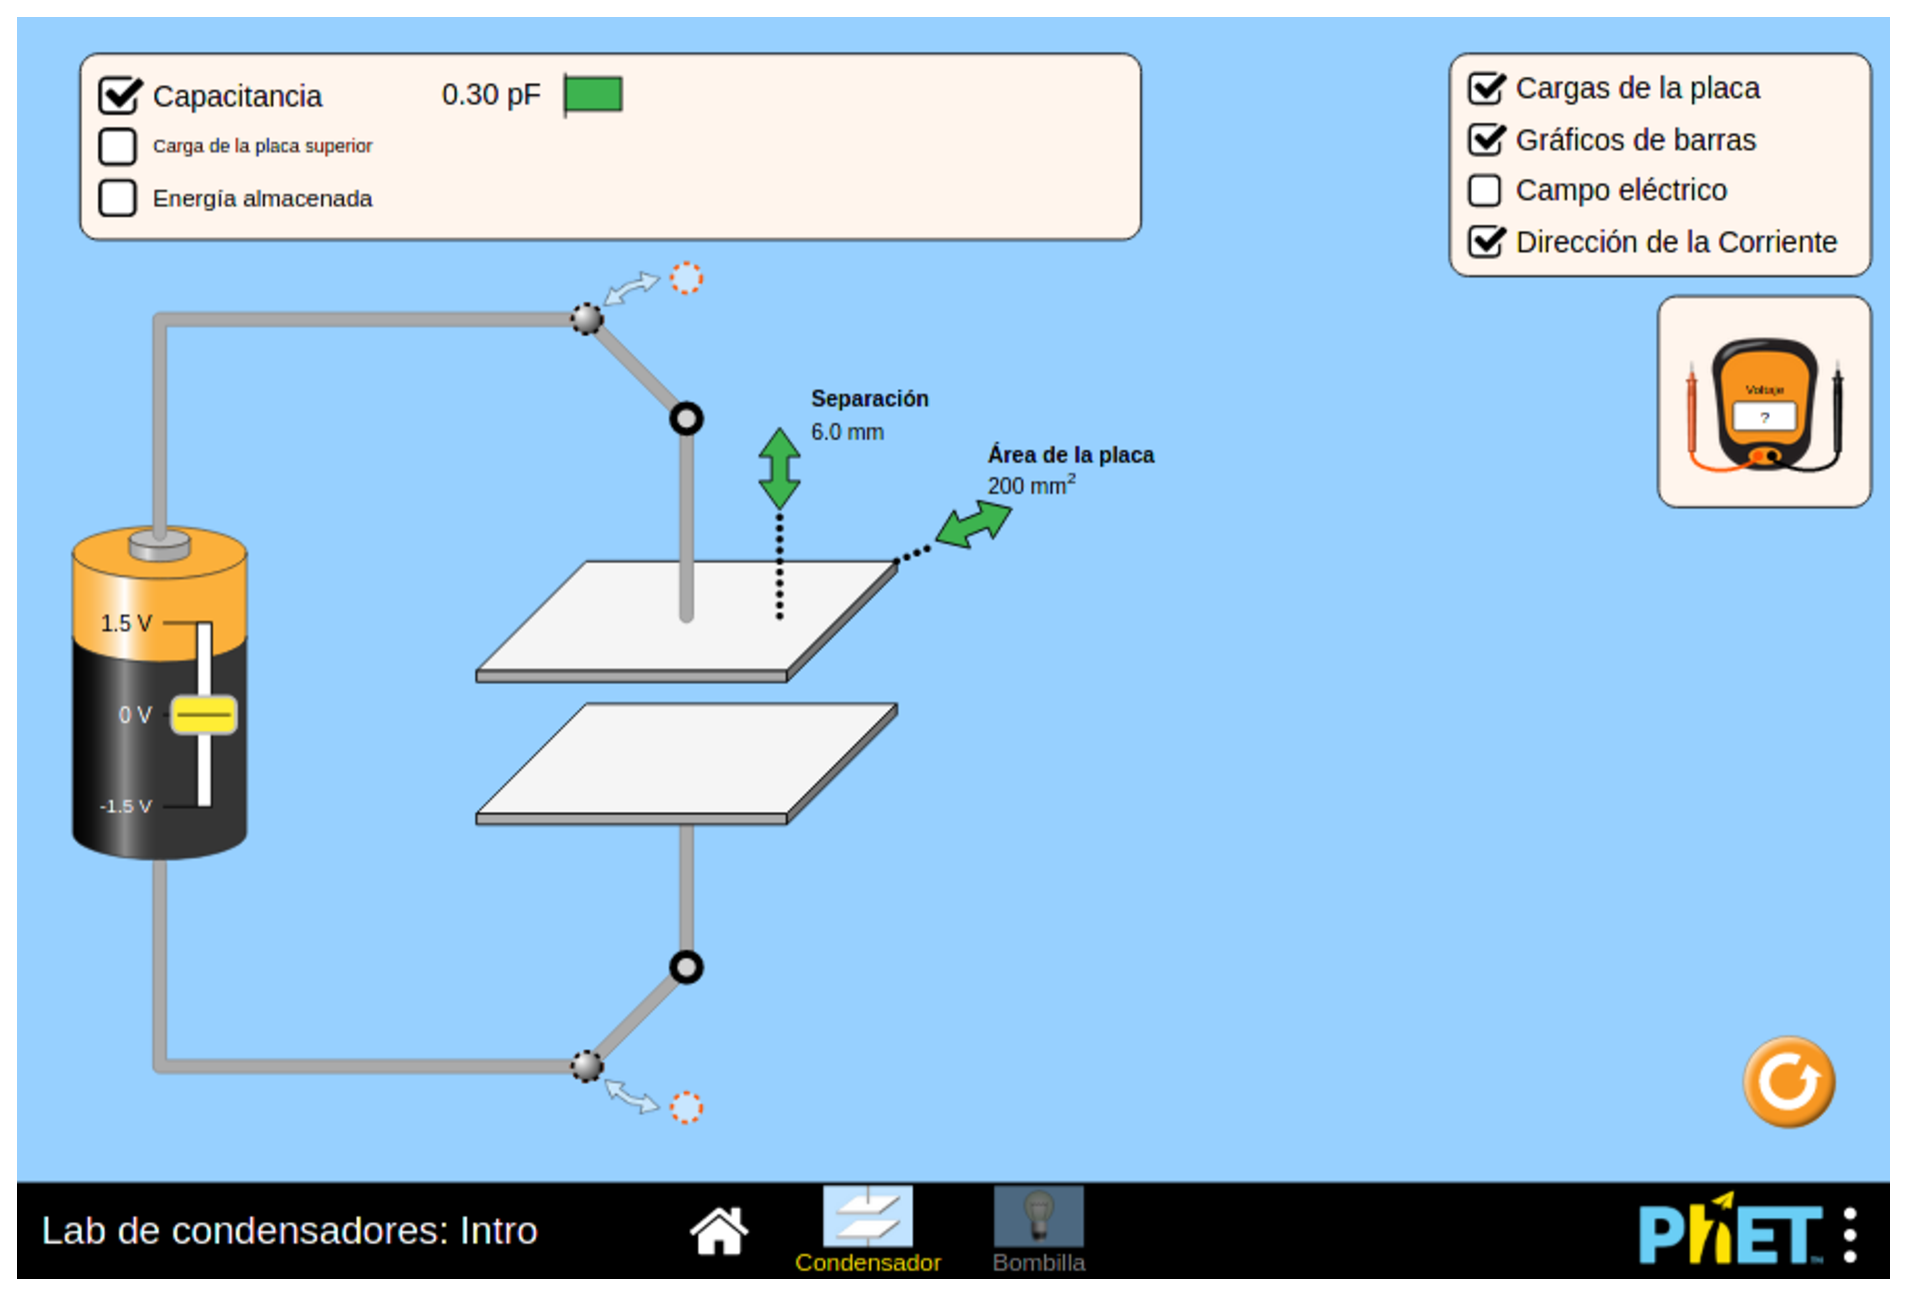
\includegraphics[scale=0.45]{resources/f3.eps}
\caption{Simulador para capacitores.}
\label{figura3}
\end{figure}

\item Establecer un valor de área $A$ de las placas del capacitor.
\item Establecer un valor de voltaje $V$ de la batería.
\item Registrar las mediciones de la capacitancia según la distancia de
    separación de las placas paralelas, y elaborar las gráficas.
\item Hallar la relación funcional entre la distancia y la capacitancia.
\item Calcular la permitividad del vacío.
\end{enumerate}

\subsection{Capacitancia en función del área}

\begin{enumerate}
\item Ir al simulador ubicado en la dirección web:
    \url{https://phet.colorado.edu/sims/html/capacitor-lab-basics/latest/capacitor-lab-basics_es.html},
        tal como se muestra en la \textbf{Figura \ref{figura3}}.
\item Establecer un valor de distancia $d$ de las placas del capacitor.
\item Establecer un valor de voltaje $V$ de la batería.
\item Registrar las mediciones de la capacitancia según el área total de la
    placa paralela, y elaborar las gráficas.
\item Hallar la relación funcional entre el área y la capacitancia.
\item Calcular la permitividad del vacío.
\end{enumerate}

\section{Resultados}

\subsection{Capacitancia en función de la distancia}

Valor del área de las placas:

\begin{equation*}
    A = 400 [mm^2]
\end{equation*}

Valor del voltaje:

\begin{equation*}
    V = 1.5 [V]
\end{equation*}

En el \textbf{Cuadro \ref{cuadro1}} se presentan los valores de las capacitancias
($C$) en función de la distancia ($d$).

\begin{table}[!h]
\begin{center}
\begin{tabular}{|c|>{\centering}m{3.0cm}<{\centering}
                  |>{\centering}m{3.0cm}<{\centering}|}
\hline
\multicolumn{3}{|c|}{$A: 400 [mm^2]$} \\
\multicolumn{3}{|c|}{$V: 1.5 [V]$} \\
\hline
$i$ & $d_i [mm]$ & $C_i [pF]$ \tabularnewline \hline
 1 & 2.0 & 1.77 \tabularnewline \hline
 2 & 2.4 & 1.48 \tabularnewline \hline
 3 & 2.6 & 1.36 \tabularnewline \hline
 4 & 2.8 & 1.26 \tabularnewline \hline
 5 & 3.0 & 1.18 \tabularnewline \hline
 6 & 3.2 & 1.11 \tabularnewline \hline
 7 & 3.4 & 1.04 \tabularnewline \hline
 8 & 3.6 & 0.98 \tabularnewline \hline
 9 & 3.8 & 0.93 \tabularnewline \hline
10 & 4.0 & 0.89 \tabularnewline \hline
11 & 4.2 & 0.84 \tabularnewline \hline
12 & 4.4 & 0.80 \tabularnewline \hline
\end{tabular}
\caption{Mediciones de la capacitancia para diferentes distancias.}
\label{cuadro1}
\end{center}
\end{table}

A partir de los datos del \textbf{Cuadro \ref{cuadro1}}, se obtiene la gráfica
presentada en la \textbf{Figura \ref{figura4}}.

\begin{figure}[!h]
\centering
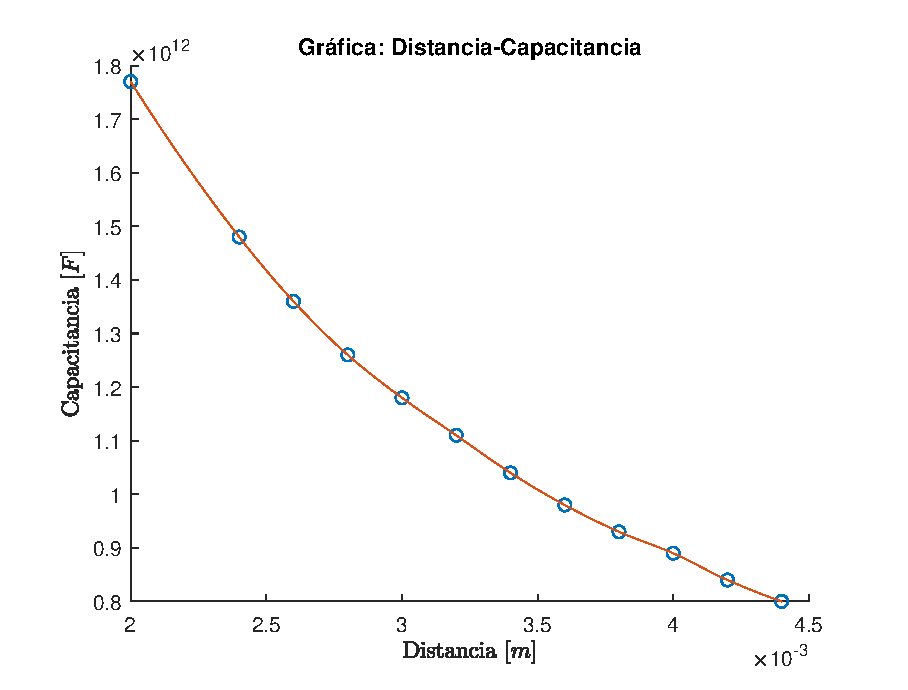
\includegraphics[scale=1.00]{resources/m1.1.eps}
\caption{Capacitancia en función de la distancia entre placas.}
\label{figura4}
\end{figure}

Por la forma de la \textbf{Figura \ref{figura4}} el modelo que se asume para la
relación funcional es:

\begin{equation*}
    C(d) = a d^b
\end{equation*}

Aplicando logaritmos a ambos lados de la ecuación obtenemos:

\begin{equation*}
    \log C = \log a + b \log d
\end{equation*}

Haciendo los siguientes cambios de variables:

\begin{equation*}
    C' = \log C
\end{equation*}
\begin{equation*}
    A = \log a
\end{equation*}
\begin{equation*}
    B = b
\end{equation*}
\begin{equation*}
    d' = \log d
\end{equation*}

Se obtiene:

\begin{equation*}
    C' = A + B d'
\end{equation*}

En el \textbf{Cuadro \ref{cuadro2}} pueden apreciarse los valores de la función
aplicando logaritmos, tales datos generan la gráfica presentada en la
\textbf{Figura \ref{figura5}}.

\begin{table}[!h]
\begin{center}
\begin{tabular}{|c|>{\centering}m{3.0cm}<{\centering}
                  |>{\centering}m{3.0cm}<{\centering}|}
\hline
$i$ & $d'_i$ & $F'_i$ \tabularnewline \hline
 1 & -6.2146 & 28.2020 \tabularnewline \hline
 2 & -6.0323 & 28.0231 \tabularnewline \hline
 3 & -5.9522 & 27.9385 \tabularnewline \hline
 4 & -5.8781 & 27.8621 \tabularnewline \hline
 5 & -5.8091 & 27.7965 \tabularnewline \hline
 6 & -5.7446 & 27.7354 \tabularnewline \hline
 7 & -5.6840 & 27.6702 \tabularnewline \hline
 8 & -5.6268 & 27.6108 \tabularnewline \hline
 9 & -5.5728 & 27.5585 \tabularnewline \hline
10 & -5.5215 & 27.5145 \tabularnewline \hline
11 & -5.4727 & 27.4567 \tabularnewline \hline
12 & -5.4262 & 27.4079 \tabularnewline \hline
\end{tabular}
\caption{Valores logaritmizados para el ajuste de curva.}
\label{cuadro2}
\end{center}
\end{table}

\begin{figure}[!h]
\centering
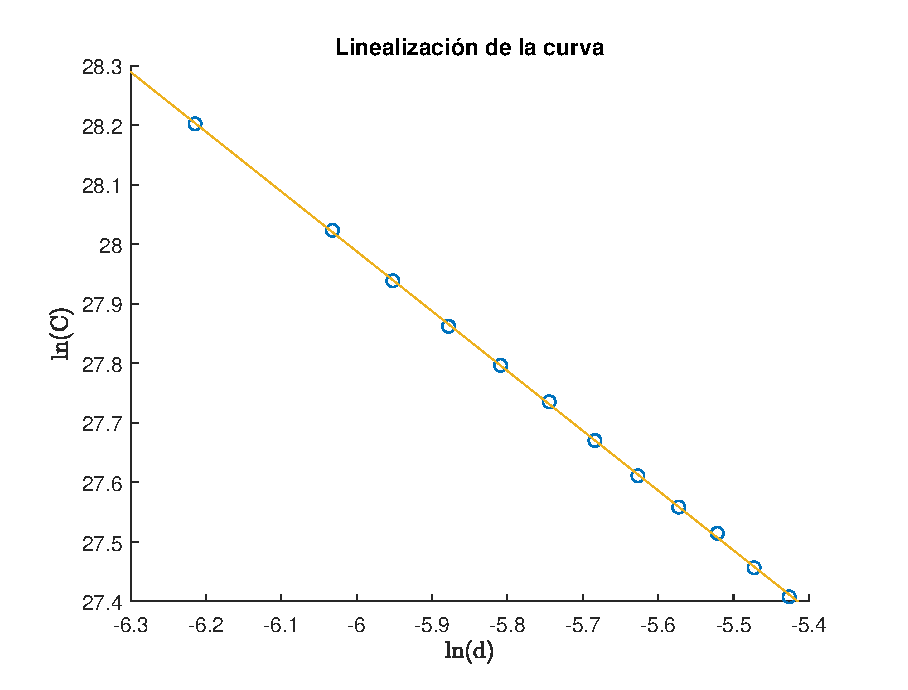
\includegraphics[scale=1.0]{resources/m1.2.eps}
\caption{Gráfica de la función linealizada.}
\label{figura5}
\end{figure}

Calculamos los parámetros de la recta por el método de los mínimos cuadrados,
con la ayuda de los datos presentados en el \textbf{Cuadro \ref{cuadro3}}.

\begin{table}[!h]
\begin{center}
\begin{tabular}{|c|>{\centering}m{1.8cm}<{\centering}
                  |>{\centering}m{1.8cm}<{\centering}
                  |>{\centering}m{1.8cm}<{\centering}
                  |>{\centering}m{1.8cm}<{\centering}
                  |>{\centering}m{1.8cm}<{\centering}
                  |>{\centering}m{2.1cm}<{\centering}|}
\hline
$i$ & $d'_i C'_i$ & $d'^2_i$ & $C'^2_i$ & $Y$ & $\delta_i$ & $\delta^2_i (\num{1e-4})$ \tabularnewline \hline
 1 & -175.2644 & 38.6214 & 795.3528 & 28.2032 & -0.0012 & 0.0151 \tabularnewline \hline
 2 & -169.0431 & 36.3885 & 785.2921 & 28.0202 &  0.0029 & 0.0825 \tabularnewline \hline
 3 & -166.2968 & 35.4292 & 780.5601 & 27.9398 & -0.0013 & 0.0176 \tabularnewline \hline
 4 & -163.7774 & 34.5525 & 776.2984 & 27.8654 & -0.0033 & 0.1091 \tabularnewline \hline
 5 & -161.4740 & 33.7461 & 772.6474 & 27.7962 &  0.0004 & 0.0013 \tabularnewline \hline
 6 & -159.3288 & 33.0005 & 769.2514 & 27.7314 &  0.0040 & 0.1601 \tabularnewline \hline
 7 & -157.2771 & 32.3076 & 765.6423 & 27.6705 & -0.0003 & 0.0008 \tabularnewline \hline
 8 & -155.3611 & 31.6611 & 762.3573 & 27.6131 & -0.0023 & 0.0536 \tabularnewline \hline
 9 & -153.5765 & 31.0556 & 759.4682 & 27.5589 & -0.0004 & 0.0016 \tabularnewline \hline
10 & -151.9202 & 30.4865 & 757.0470 & 27.5074 &  0.0071 & 0.5079 \tabularnewline \hline
11 & -150.2613 & 29.9501 & 753.8686 & 27.4584 & -0.0017 & 0.0293 \tabularnewline \hline
12 & -148.7193 & 29.4431 & 751.1918 & 27.4117 & -0.0038 & 0.1443 \tabularnewline \hline
\end{tabular}
\caption{Valores para el método de mínimos cuadrados.}
\label{cuadro3}
\end{center}
\end{table}

\begin{equation*}
    n = 12
\end{equation*}
\begin{equation*}
    \sum d'_i = -68.9349
\end{equation*}
\begin{equation*}
    \sum C'_i = 332.7762
\end{equation*}
\begin{equation*}
    \sum d'^2_i = 396.6422
\end{equation*}
\begin{equation*}
    \sum C'^2_i = \num{9.2290e3}
\end{equation*}
\begin{equation*}
    \sum d'_i C'_i = \num{-1.9123e3}
\end{equation*}
\begin{equation*}
    \Delta_1 = n \sum d'^2_i - \left( \sum d'_i \right)^2 = 7.6921
\end{equation*}
\begin{equation*}
    \Delta_2 = n \sum C'^2_i - \left( \sum C'_i \right)^2 = 7.7539
\end{equation*}
\begin{equation*}
    A = \frac{\sum C'_i \sum d'^2_i - \sum d'_i C'_i \sum d'_i}{\Delta_1} = 21.9642
\end{equation*}
\begin{equation*}
    B = \frac{n \sum d'_i C'_i - \sum d'_i \sum C'_i}{\Delta_1} = -1.0039
\end{equation*}
\begin{equation*}
    \sum \delta^2 = \num{1.1232e-4}
\end{equation*}
\begin{equation*}
    \sigma^2 = \frac{\sum \delta^2_i}{n-2} = \num{1.1232e-5}
\end{equation*}
\begin{equation*}
    \sigma_A = \sqrt{\frac{\sigma^2 \sum d'^2_i}{\Delta_1}} = 0.0241
\end{equation*}
\begin{equation*}
    \sigma_B = \sqrt{\frac{\sigma^2 n}{\Delta_1}} = 0.0042
\end{equation*}

\begin{equation*}
    A = (21.9642 \pm 0.0241)[u]; 0.1096%
\end{equation*}
\begin{equation*}
    B = (-1.0039 \pm 0.0042)[u]; 0.4170\%
\end{equation*}

Siendo el coeficiente de correlación:

\begin{equation*}
    R = \frac{n \sum d'_i C'_i - (\sum d'_i)(\sum C'_i)}{\sqrt{\Delta_1 \Delta_2}} = -0.9999
\end{equation*}

La ecuación de la recta resultante es:

\begin{equation*}
    C' = 21.9642 - 1.0039 d'
\end{equation*}

A partir de los parámetros de recta $A$ y $B$, calculamos los parámetros $a$ y
$b$ de la curva original y sus errores por el método de propagación de errores:

\begin{equation*}
    a = e^{A} = e^{21.9642} = \num{3.4589e9}
\end{equation*}
\begin{equation*}
    b = B = -1.0039
\end{equation*}
\begin{equation*}
    e_a = e^A e_A = e^{21.9642} \num{0.0241} = \num{8.3244e7}
\end{equation*}
\begin{equation*}
    e_b = e_B = 0.0042
\end{equation*}

Obteniendo finalmente los valores de la curva:

\begin{equation*}
    a = (\num{3.4589e9} \pm \num{8.3244e7})[C^2/N]; 2.4066\%
\end{equation*}
\begin{equation*}
    b = (-1.0039 \pm 0.0042)[u]; 0.4170\%
\end{equation*}

La ecuación de la curva resultante es:

\begin{equation}
    C(d) = a d^b = \num{3.4589e9} d^{-1.0039} = \frac{\num{3.4589e9}}{d}
\label{curva}
\end{equation}

Se comprueba la relación entre la capacitancia y la distancia de separación
entre placas descrito por la \textbf{Ecuación (\ref{capacitancia})}.

\begin{center}
\begin{tabular}{|>{\centering}m{9.2cm}<{\centering}|}
\hline
\textbf{Resultado} 
\tabularnewline \hline
\\
\Large{$C \propto \frac{1}{d}$} \tabularnewline
\\
\hline
\end{tabular}
\end{center}

Comparando la \textbf{Ecuación (\ref{capacitancia})} con la ecuación de la
curva, se determina el valor de la permitividad del vacío con su respectivo
error:

\begin{center}
\begin{tabular}{|>{\centering}m{12.0cm}<{\centering}|}
\hline
\textbf{Resultado}
\tabularnewline \hline
\\
    $\epsilon_0 = \frac{a}{A} = (\num{8.6474e12} \pm \num{1.7996e24}) [C^2/m^2 N]; \num{2.0811e13} \%$ \tabularnewline
\\
\hline
\end{tabular}
\end{center}

\subsection{Capacitancia en función del área}

Valor de la distancia de separación entre placas:

\begin{equation*}
    d = 2.0 [mm]
\end{equation*}

Valor del voltaje:

\begin{equation*}
    V = 1.5 [V]
\end{equation*}

En el \textbf{Cuadro \ref{cuadro4}} se presentan los valores de las capacitancias
($C$) en función del área ($A$).

\begin{table}[!h]
\begin{center}
\begin{tabular}{|c|>{\centering}m{3.0cm}<{\centering}
                  |>{\centering}m{3.0cm}<{\centering}|}
\hline
\multicolumn{3}{|c|}{$d: 2.0 [mm]$} \\
\multicolumn{3}{|c|}{$V: 1.5 [V]$} \\
\hline
$i$ & $a_i [mm^2]$ & $C_i [pF]$ \tabularnewline \hline
 1 & 400 & 1.77 \tabularnewline \hline
 2 & 390 & 1.73 \tabularnewline \hline
 3 & 380 & 1.68 \tabularnewline \hline
 4 & 370 & 1.64 \tabularnewline \hline
 5 & 360 & 1.59 \tabularnewline \hline
 6 & 350 & 1.55 \tabularnewline \hline
 7 & 340 & 1.51 \tabularnewline \hline
 8 & 330 & 1.46 \tabularnewline \hline
 9 & 320 & 1.42 \tabularnewline \hline
10 & 310 & 1.37 \tabularnewline \hline
11 & 300 & 1.33 \tabularnewline \hline
12 & 290 & 1.28 \tabularnewline \hline
\end{tabular}
\caption{Mediciones de la capacitancia para diferentes áreas.}
\label{cuadro4}
\end{center}
\end{table}

A partir de los datos del \textbf{Cuadro \ref{cuadro4}}, se obtiene la gráfica
presentada en la \textbf{Figura \ref{figura6}}.

\begin{figure}[!h]
\centering
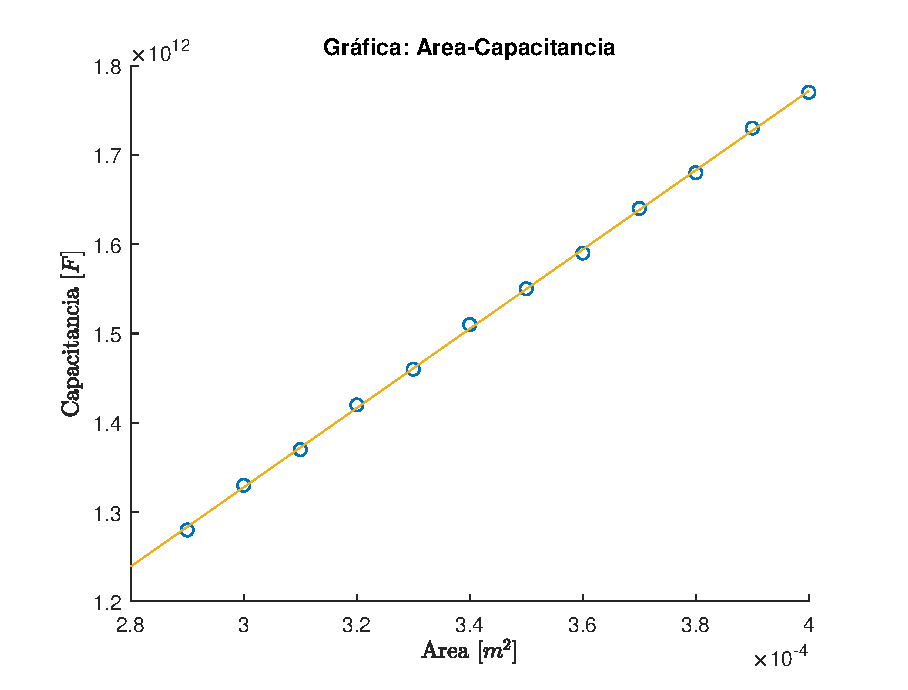
\includegraphics[scale=1.00]{resources/m2.eps}
\caption{Capacitancia en función del área del capacitor.}
\label{figura6}
\end{figure}

Por tanto, la ecuación de ajuste es:

\begin{equation*}
    C(a) = A + B a
\end{equation*}

Se calcularon los parámetros de la recta por el método de los mínimos cuadrados,
con la ayuda de los datos presentados en el \textbf{Cuadro \ref{cuadro5}}.

\begin{table}[!h]
\begin{center}
\begin{tabular}{|c|>{\centering}m{2.1cm}<{\centering}
                  |>{\centering}m{2.0cm}<{\centering}
                  |>{\centering}m{2.1cm}<{\centering}
                  |>{\centering}m{1.9cm}<{\centering}
                  |>{\centering}m{2.0cm}<{\centering}
                  |>{\centering}m{2.0cm}<{\centering}|}
\hline
$i$ & $a_i C'_i (\num{1e8})$ & $a^2_i (\num{1e-6})$ & $C^2_i (\num{1e-6})$ & $Y (\num{1e12})$ & $\delta_i (\num{1e9})$ & $\delta^2_i (\num{1e19})$ \tabularnewline \hline
 1 & 7.0800 & 0.1600 & 3.1329 & 1.7715 & -1.5385 & 0.2367 \tabularnewline \hline
 2 & 6.7470 & 0.1521 & 2.9929 & 1.7272 &  2.8322 & 0.8021 \tabularnewline \hline
 3 & 6.3840 & 0.1444 & 2.8224 & 1.6828 & -2.7972 & 0.7824 \tabularnewline \hline
 4 & 6.0680 & 0.1369 & 2.6896 & 1.6384 &  1.5734 & 0.2476 \tabularnewline \hline
 5 & 5.7240 & 0.1296 & 2.5281 & 1.5941 & -4.0559 & 1.6451 \tabularnewline \hline
 6 & 5.4250 & 0.1225 & 2.4025 & 1.5497 &  0.3147 & 0.0099 \tabularnewline \hline
 7 & 5.1340 & 0.1156 & 2.2801 & 1.5053 &  4.6853 & 2.1952 \tabularnewline \hline
 8 & 4.8180 & 0.1089 & 2.1316 & 1.4609 & -0.9441 & 0.0891 \tabularnewline \hline
 9 & 4.5440 & 0.1024 & 2.0164 & 1.4166 &  3.4266 & 1.1741 \tabularnewline \hline
10 & 4.2470 & 0.0961 & 1.8769 & 1.3722 & -2.2028 & 0.4852 \tabularnewline \hline
11 & 3.9900 & 0.0900 & 1.7689 & 1.3278 &  2.1678 & 0.4699 \tabularnewline \hline
12 & 3.7120 & 0.0841 & 1.6384 & 1.2835 & -3.4615 & 1.1982 \tabularnewline \hline
\end{tabular}
\caption{Valores para el método de mínimos cuadrados.}
\label{cuadro5}
\end{center}
\end{table}

\begin{equation*}
    n = 12
\end{equation*}
\begin{equation*}
    \sum a_i = 0.0041
\end{equation*}
\begin{equation*}
    \sum C_i = \num{1.8330e13}
\end{equation*}
\begin{equation*}
    \sum a^2_i = \num{1.4426e-6}
\end{equation*}
\begin{equation*}
    \sum C^2_i = \num{2.8281e25}
\end{equation*}
\begin{equation*}
    \sum a_i C_i = \num{6.3873e9}
\end{equation*}
\begin{equation*}
    \Delta_1 = n \sum a^2_i - \left( \sum a_i \right)^2 = \num{1.7160e-7}
\end{equation*}
\begin{equation*}
    \Delta_2 = n \sum C^2_i - \left( \sum C_i \right)^2 = \num{3.3795e24}
\end{equation*}
\begin{equation*}
    A = \frac{\sum C_i \sum a^2_i - \sum a_i C_i \sum a_i}{\Delta_1} = \num{-3.2867e9}
\end{equation*}
\begin{equation*}
    B = \frac{n \sum a_i C_i - \sum a_i \sum C_i}{\Delta_1} = \num{4.4371e15}
\end{equation*}
\begin{equation*}
    \sum \delta^2 = \num{9.3357e19}
\end{equation*}
\begin{equation*}
    \sigma^2 = \frac{\sum \delta^2_i}{n-2} = \num{9.3357e18}
\end{equation*}
\begin{equation*}
    \sigma_A = \sqrt{\frac{\sigma^2 \sum a^2_i}{\Delta_1}} = \num{8.8590e9}
\end{equation*}
\begin{equation*}
    \sigma_B = \sqrt{\frac{\sigma^2 n}{\Delta_1}} = \num{2.5551e13}
\end{equation*}

\begin{equation*}
    A = (\num{-3.2867e9} \pm \num{8.8590e9})[F]; 269.5412\%
\end{equation*}
\begin{equation*}
    B = (\num{4.4371e15} \pm \num{2.5551e13})[C^2/m^3 N]; 0.5758\%
\end{equation*}

Siendo el coeficiente de correlación:

\begin{equation*}
    R = \frac{n \sum a_i C_i - (\sum a_i)(\sum C_i)}{\sqrt{\Delta_1 \Delta_2}} = 0.9998
\end{equation*}

La ecuación de la recta resultante es:

\begin{equation*}
    C(a) = \num{-3.2867e9} + \num{4.4371e15} a
\end{equation*}

Se comprueba la relación entre la capacitancia y el área de las placas descrito
por la \textbf{Ecuación (\ref{capacitancia})}.

\begin{center}
\begin{tabular}{|>{\centering}m{9.2cm}<{\centering}|}
\hline
\textbf{Resultado} 
\tabularnewline \hline
\\
\Large{$C \propto a$} \tabularnewline
\\
\hline
\end{tabular}
\end{center}

Comparando la \textbf{Ecuación (\ref{capacitancia})} con la ecuación de la
curva, se determina el valor de la permitividad del vacío con su respectivo
error:

\begin{center}
\begin{tabular}{|>{\centering}m{12.0cm}<{\centering}|}
\hline
\textbf{Resultado}
\tabularnewline \hline
\\
    $\epsilon_0 = d B = (\num{8.8741e12} \pm \num{8.8888e11}) [C^2/m^2 N]; 10.0166\%$ \tabularnewline
\\
\hline
\end{tabular}
\end{center}

\section{Conclusiones}

Se realizó la gráfica de la capacitancia y el ajuste de curva, tanto como
función de la distancia de separación entre placas, como del área de la placa,
comprobando las relaciones funcionales de la teoría planteada.

Además se halló el valor de la permitividad del vacío, siendo esta muy próximo
al valor teórico para ambos casos.

\begin{thebibliography}{99}

\bibitem{UCL} CAPACITANCIA. CONDENSADOR DE PLACAS PARALELAS. CONEXIÓN DE CONDENSADORES \\
Extraído el 20 de Abril del 2021, de: \\
\url{http://www.fisica.ucn.cl/wp-content/uploads/2016/03/DAFI219-03-Capacitancia.pdf}.
 
\bibitem{Sears y Zemansky} Sears y Zemansky (2013).\\
Física Universitaria. Volumen 1.\\
13va Edición.\\
Capitulo 11.

\end{thebibliography}

\end{document}

